%%
%% This is file `mcmthesis-demo.tex',
%% generated with the docstrip utility.
%%
%% The original source files were:
%%
%% mcmthesis.dtx  (with options: `demo')
%% 
%% -----------------------------------
%% 
%% This is a generated file.
%% 
%% Copyright (C)
%%     2010 -- 2015    by Zhaoli Wang
%%     2014 -- present by Liam Huang
%% 
%% This work may be distributed and/or modified under the
%% conditions of the LaTeX Project Public License, either version 1.3
%% of this license or (at your option) any later version.
%% The latest version of this license is in
%%   http://www.latex-project.org/lppl.txt
%% and version 1.3 or later is part of all distributions of LaTeX
%% version 2005/12/01 or later.
%% 
%% This work has the LPPL maintenance status `maintained'.
%% 
%% The Current Maintainer of this work is Liam Huang.
%% 
\documentclass{mcmthesis}
\mcmsetup{CTeX = false,   % 使用 CTeX 套装时,设置为 true
        tcn = 2001560, problem = C,
        sheet = true, titleinsheet = true, keywordsinsheet = false,
        titlepage = false, abstract = true}
\usepackage{palatino}
\usepackage{lipsum}

\title{A Wealth of Data}
\author{\small \href{http://www.latexstudio.net/}
  {
\includegraphics[width=7cm]{mcmthesis-logo}}}
\date{\today}
\begin{document}
\begin{abstract}
  \lipsum[1]
\end{abstract}
\maketitle
%% Generate the Table of Contents, if it's needed.
\tableofcontents
\newpage
%%
%% Generate the Memorandum, if it's needed.
\memoto{Marketing Director of Sunshine Company}
\memofrom{MCM Team \#2001560}
\memosubject{Data Analysis Results}
\memodate{\today}
% \logo{\LARGE I'm pretending to be a LOGO!}
\begin{memo}[Letter]
  \lipsum[1]
\end{memo}

\section{Introduction}
\subsection{Background}
In recent years, more and more customers choose to shop online for its less space-time limitation and the convinent home delivery service. However, compared to the traditional physical stores, customers can only assess products by the privided profile and pictures instead of seeing the real ones. The information gap here is one of the main causes of dissatisfied purchases. To help comsumers know the product better, many online marketplace platforms, such as Amazon, introduce "review system". Customers are provided with an opportunity to express their level of satisfaction and further opinions or information about the products they have bought through rating and reviewing. Those additional information can assist other customers' purchasing decision. Meanwhile, it also help companies to gain insights into the market they participate and improve their product design.

But we found that not all reviews are equally relevant. Some reviews are too general; some people's ratings don’t match their reviews; there are even deliberately misleading reviews, such as malicious defamation from competitors or the praise by the bribed reviewers. Therefore, when using data to assist business decisions, we need to analyze data carefully and comprehensively to obtain more accurate results. More factors should be considered, such as the ratings, review contents and review time, rather than simply  calculate the average rating level.
\subsection{Problem Restatement}
\subsection{Data Source}
Our model is informed by the customer-supplied ratings and reviews for microwave ovens, baby pacifiers, and hair dryers sold in the Amazon marketplace over more than 10 years.

\section{Assumptions}
\begin{itemize}
  \item 
\end{itemize}

\section{Nomenclature}
\begin{table}[h]
  \centering
  \begin{tabular}{ccc}
    \hline
    Symbol & Definition\\
    \hline
    Steve Jobs& 001\\
    \hline
  \end{tabular}
  \caption{variables and functions}
\end{table}

\section{ Model Design }

\section{ Part \uppercase\expandafter{\romannumeral1}:  }

\section{ Part \uppercase\expandafter{\romannumeral2}:  }

\section{Sensitivity Analysis}

\section{Conclusions}
\subsection{Strengths}
\begin{itemize}
  \item \textbf{Applies widely}\\
        This  system can be used for many types of airplanes, and it also
        solves the interference during  the procedure of the boarding
        airplane,as described above we can get to the  optimization
        boarding time.We also know that all the service is automate.
  \item \textbf{Improve the quality of the airport service}\\
        Balancing the cost of the cost and the benefit, it will bring in
        more convenient  for airport and passengers.It also saves many
        human resources for the airline. \item \textbf{}
\end{itemize}

\begin{figure}[h]
  \small
  \centering
  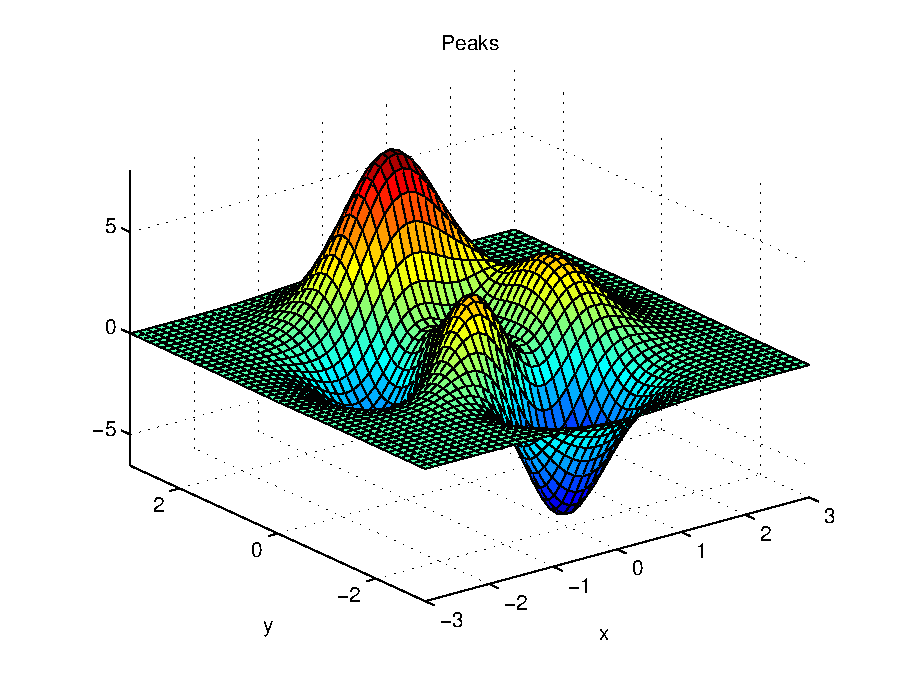
\includegraphics[width=12cm]{mcmthesis-aaa.eps}
  \caption{aa} \label{fig:aa}
\end{figure}

\lipsum[8] \eqref{aa}
\begin{equation}
  a^2 \label{aa}
\end{equation}


\[
  p_{j}=\begin{cases} 0,              & \text{if $j$ is odd}  \\
    r!\,(-1)^{j/2}, & \text{if $j$ is even}
  \end{cases}
\]

%% References
\begin{thebibliography}{99}
  \bibitem{1} D.~E. KNUTH   The \TeX{}book  the American
  Mathematical Society and Addison-Wesley
  Publishing Company , 1984-1986.
  \bibitem{2}Lamport, Leslie,  \LaTeX{}: `` A Document Preparation System '',
  Addison-Wesley Publishing Company, 1986.
  \bibitem{3}\url{http://www.latexstudio.net/}
  \bibitem{4}\url{http://www.chinatex.org/}
\end{thebibliography}

\begin{appendices}

  \section{First appendix}

  \lipsum[13]

  Here are simulation programmes we used in our model as follow.\\

  \textbf{\textcolor[rgb]{0.98,0.00,0.00}{Input matlab source:}}
  \lstinputlisting[language=Matlab]{./code/mcmthesis-matlab1.m}

  \section{Second appendix}

  some more text \textcolor[rgb]{0.98,0.00,0.00}{\textbf{Input C++ source:}}
  \lstinputlisting[language=C++]{./code/mcmthesis-sudoku.cpp}

\end{appendices}
\end{document}

%% 
%% This work consists of these files mcmthesis.dtx,
%%                                   figures/ and
%%                                   code/,
%% and the derived files             mcmthesis.cls,
%%                                   mcmthesis-demo.tex,
%%                                   README,
%%                                   LICENSE,
%%                                   mcmthesis.pdf and
%%                                   mcmthesis-demo.pdf.
%%
%% End of file `mcmthesis-demo.tex'.
